\documentclass[10pt,border=2pt]{standalone}
\usepackage{times}
\usepackage{amsmath}
\usepackage{pgfplots}
\pgfplotsset{compat=1.18}

\definecolor{samcolor}{HTML}{1F4E79}
\definecolor{headcolor}{HTML}{C55A11}
\definecolor{gridgray}{HTML}{DADADA}

\begin{document}
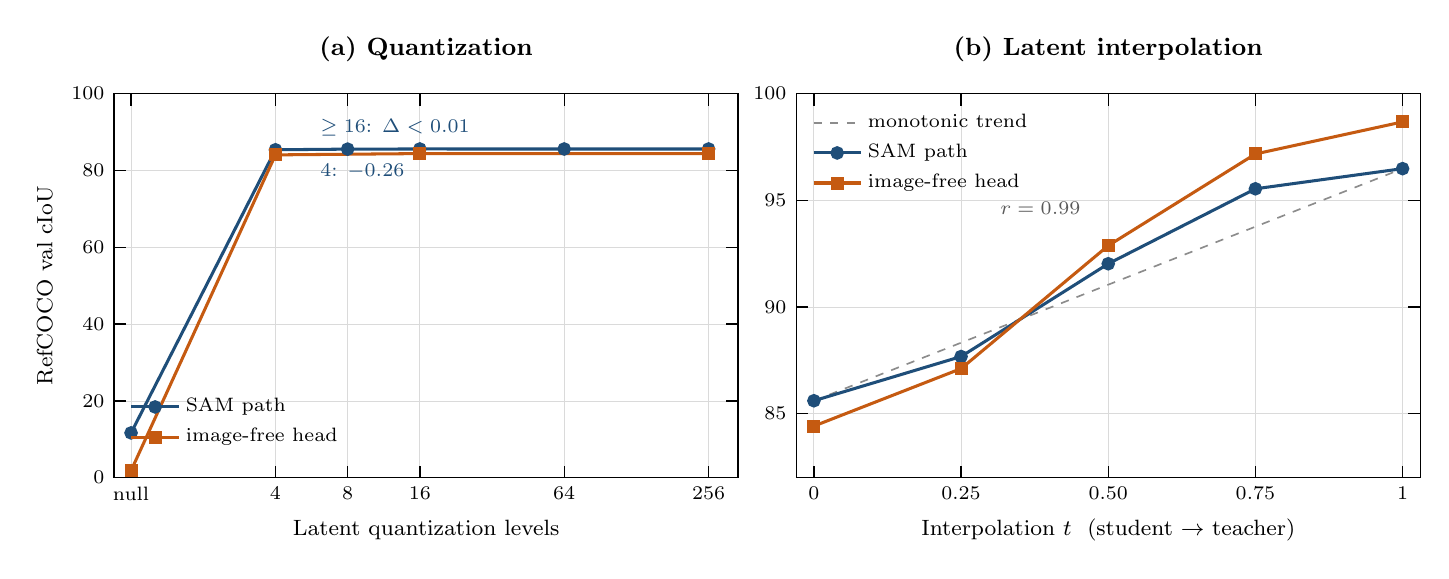
\begin{tikzpicture}

% ============================================================
% (a) Quantization sweep -- x is log2, "null" sits at 1
% ============================================================
\begin{axis}[
  name=quant,
  width=3.12in, height=1.92in,
  scale only axis,
  xmode=log, log basis x=2,
  xmin=0.85, xmax=340,
  ymin=0, ymax=100,
  xtick={1,4,8,16,64,256},
  xticklabels={{null},4,8,16,64,256},
  xlabel={Latent quantization levels},
  ylabel={RefCOCO val cIoU},
  title={(a) Quantization},
  title style={font=\small\bfseries, yshift=2pt},
  label style={font=\footnotesize},
  tick label style={font=\scriptsize},
  grid=major,
  grid style={gridgray, line width=0.3pt},
  axis line style={black, line width=0.5pt},
  tick style={black, line width=0.5pt},
  legend style={font=\scriptsize, draw=none, fill=none,
                at={(0.02,0.06)}, anchor=south west,
                legend cell align=left, row sep=0.5pt,
                inner sep=1pt},
]

\addplot[color=samcolor, line width=1.1pt, mark=*, mark size=1.9pt,
         mark options={fill=samcolor, draw=samcolor}]
  coordinates {(1,11.669) (4,85.402) (8,85.570) (16,85.609) (64,85.607) (256,85.608)};
\addlegendentry{SAM path}

\addplot[color=headcolor, line width=1.1pt, mark=square*, mark size=1.8pt,
         mark options={fill=headcolor, draw=headcolor}]
  coordinates {(1,1.85) (4,84.07) (16,84.41) (256,84.42)};
\addlegendentry{image-free head}

\node[font=\scriptsize, anchor=south west, text=samcolor]
  at (axis cs:5.6,86.4) {$\geq 16$: $\Delta<0.01$};
\node[font=\scriptsize, anchor=north west, text=samcolor]
  at (axis cs:5.6,84.2) {$4$: $-0.26$};
\end{axis}

% ============================================================
% (b) Interpolation along the student -> teacher geodesic
% ============================================================
\begin{axis}[
  name=interp,
  at={(quant.east)}, anchor=west, xshift=21pt,
  width=3.12in, height=1.92in,
  scale only axis,
  xmin=-0.03, xmax=1.03,
  ymin=82, ymax=100,
  xtick={0,0.25,0.5,0.75,1},
  xticklabels={0,0.25,0.50,0.75,1},
  xlabel={Interpolation $t$ \ (student $\rightarrow$ teacher)},
  title={(b) Latent interpolation},
  title style={font=\small\bfseries, yshift=2pt},
  label style={font=\footnotesize},
  tick label style={font=\scriptsize},
  grid=major,
  grid style={gridgray, line width=0.3pt},
  axis line style={black, line width=0.5pt},
  tick style={black, line width=0.5pt},
  legend style={font=\scriptsize, draw=none, fill=none,
                at={(0.02,0.97)}, anchor=north west,
                legend cell align=left, row sep=0.5pt,
                inner sep=1pt},
]

\addplot[color=black!45, line width=0.6pt, dashed, domain=0:1, samples=2]
  {85.608 + (96.488-85.608)*x};
\addlegendentry{monotonic trend}

\addplot[color=samcolor, line width=1.1pt, mark=*, mark size=1.9pt,
         mark options={fill=samcolor, draw=samcolor}]
  coordinates {(0,85.608) (0.25,87.680) (0.5,92.030) (0.75,95.543) (1,96.488)};
\addlegendentry{SAM path}

\addplot[color=headcolor, line width=1.1pt, mark=square*, mark size=1.8pt,
         mark options={fill=headcolor, draw=headcolor}]
  coordinates {(0,84.421) (0.25,87.114) (0.5,92.879) (0.75,97.176) (1,98.679)};
\addlegendentry{image-free head}

\node[font=\scriptsize, anchor=south west, text=black!65]
  at (axis cs:0.30,93.9) {$r=0.99$};

\end{axis}

\end{tikzpicture}
\end{document}
